

\chapter{Laser-based Orientation}
In this...

\section{Projections}
The use of some regular and known geometrical shape that could be projected onto the net for use for orientation 
was early put forward. The idea behind this is based on the work by \citet{carlsen10}, who used 
a set of line lasers for \todo{Hva var dette egentlig?}

\section{Patterns}
There are many different patterns that may give more information about 
orientation of the ROV relative to the net than some simple lines. The 
different polygons in figure \vref{fig:pattern_triangle} to \vref{fig:pattern_heptagon}
were chosen as a good start for further investigation together with the 
circle as shown in \vref{fig:pattern_circle}.

\begin{figure}[htbp]
	\subfloat[Triangle]{
		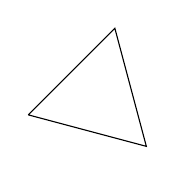
\begin{tikzpicture}[scale=0.1]
			\draw (0,4) -- (11,15) -- (15,0) -- (0,4);
		\end{tikzpicture}\label{fig:pattern_triangle}
	}\hfill
	\subfloat[Square]{
		\begin{tikzpicture}[scale=0.1]
			\draw (0,0) -- (0,15) -- (15,15) -- (15,0) -- (0,0);
		\end{tikzpicture}\label{fig:pattern_square}
	}\hfill
	\subfloat[Pentagon]{
		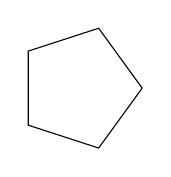
\begin{tikzpicture}[scale=1]
			\newdimen\R
			\R=0.8cm
			\draw (0:\R)
				\foreach \x in {72,144,...,360} {  -- (\x:\R) };
		\end{tikzpicture}\label{fig:pattern_pentagon}
	}
	\\
	\subfloat[Hexagon]{
		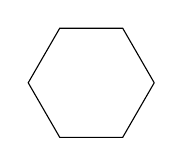
\begin{tikzpicture}[scale=1]
			\newdimen\R
			\R=0.8cm
			\draw (0:\R)
				\foreach \x in {60,120,...,360} {  -- (\x:\R) };
		\end{tikzpicture}\label{fig:pattern_hexagon}
	}\hfill
	\subfloat[Heptagon]{
		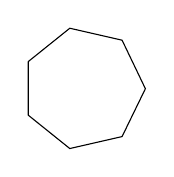
\begin{tikzpicture}[scale=0.8]
			\draw (-0.76,1.54) -- (-0.76,0.69) -- (-0.10,0.16) -- (0.73,0.35) -- (1.1,1.11) -- (0.73,1.88) -- (-0.10,2.07) -- (-0.76,1.54);
		\end{tikzpicture}\label{fig:pattern_heptagon}
	}\hfill
	\subfloat[Circle]{
		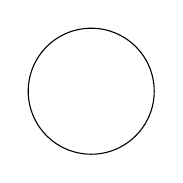
\begin{tikzpicture}[scale=0.8]
			\draw (0,0) circle(1);
		\end{tikzpicture}\label{fig:pattern_circle}
	}
	\caption{Different laser patterns}
	\label{fig:laser_pattern}
\end{figure}

Criteria for a good pattern should contain
\begin{enumerate}
	\item Not ambiguous when interpolating lines
	\item Easy algorithm to reconstruct shape
	\item Try to give orientation information\footnote{Avoid aperture problem, see section \vref{sec:aperture.problem}}
\end{enumerate}

It can be shown that amongst the patterns in figure \vref{fig:laser_pattern} that all patterns with a even number 
of vertices is prone to the aperture problem. This means that pattern \ref{fig:pattern_square} 
and \ref{fig:pattern_hexagon} can be eliminated right away. Looking at the pentagon and heptagon, they 
have respectively $\frac{\SI{360}{\degree}}{5} = \SI{72}{\degree}$ and $\frac{\SI{360}{\degree}}{7} \approx \SI{51.4}{\degree}$ angle 
for each corner, and the angles get closer as the number of vertices increases.

The best choice seems to be either a triangle or a circle. The triangle is easy to reconstruct. Only two of the vertices 
needs to be known to do a full reconstruction if the angles of the triangle is known. The orientation can 
also be determined within a third of a full revolution without ambiguity. However, the triangle 
gives ambiguity each $\pm$\SI{60}{\degree}, so the problem of ambiguous orientation can not be solved using a 
regular pattern.

Irregular patterns are also possible, and using a irregular pattern would remove all ambiguity of the operation. A irregular 
pattern is however much more difficult to recreate out of partial lines. Due to this added complexity, a simple circle turns out 
to be the best choice.

A circle can not convey any orientation data, as there are no corners and vertices to link a angle to the net onto which it is projected.
It can however give information on distance to the net by checking the amount of masks in the net that is inside the circle. The 
deformation of the circle will also give information on the tilt of the ROV relative to the net. The shape that would be read back in 
this case would be a ellipsis. The ration of the minor- and major axis in the ellipsis would give estimates on these angles. 

Ellipsis are quite easy to detect using computer vision. The most used algorithm is described in \citet{fitzgibbon95}. This algorithm fits a ellipsis onto a set of points, usually >5 is needed. The algorithm optimizes the error of the found ellipsis for all 
points. The error would then be a measure of the deformation caused by movement in the net.

\begin{figure}[htbp]
    \centering
    \subfloat[Simulated points]{\label{fig:ellipsis_1}{\includegraphics[width=1\textwidth]{ellipsis_1}}}
    \\
    \subfloat[Detected ellipsis]{\label{fig:ellipsis_2}{\includegraphics[width=1\textwidth]{ellipsis_2}}}
	\caption{Simulation of a projected ellipsis and the detected ellipsis. Blue point sets are set to vibrate in a random pattern, green dot is the detected point and blue circle is the fitted ellipsis.}
	\label{fig:ellipsis}
\end{figure}

The implementation shown in figure \vref{fig:ellipsis} proved to be quite accurate and stable.
A test pattern was generated where a random number of points were laid out on a 
elliptical path where the points were allowed to move in all directions. As figure \vref{fig:ellipsis_2} shows, points 
that diverge much from the elliptical path does not affect the found ellipsis in a great deal.

\section{Algorithm}
The algorithm used to generate the ellipsis in \vref{fig:ellipsis_2} is based on a chain of standard 
computer vision algorithms and filters. The chain consists of

\begin{enumerate}
	\item Color conversion to grayscale.
	\item Gaussian smoothing. See section \vref{sec:gaussian.filter}.
	\item Detection of points using the Hough Circle algorithm. See section \vref{sec:hough.circles}.
	\item Discarding of points outside the ROI.
	\item Use the \citet{fitzgibbon95} algorithm to fit a ellipsis over the remaining points.
\end{enumerate}

\section{Hardware}
To manufacture the hardware, a specification were developed together with Diode Laser Concepts, INC\footnote{\url{www.diodelaserconcepts.com}}. This is a reseller that 
specializes in all sorts of laser equipment, and has been use by the institute before. It turned out that circular laser 
are not a normal configuration, so after some discussion we were referred to Frankfurt Laser Company\footnote{\url{www.frlaserco.com}} which 
is a laser manufacturer based in Europe.

After even more discussions with Frankfurt Laser Company, it became clear that manufacturing such a specialized laser as the one 
required would be difficult. The first quote had a minimum order of 1,500 units. Due to the high manufacturing cost for single 
units, the efforts for acquiring a laser were cancelled.

The lack of laser hardware means that the algorithm used to detect ellipsis was never proven to work outside of simulations. Real life 
data on the performance of the detector were therefore not available. However, based on the dynamic simulations, the ellipsis were always 
detected successfully. The quality of the fitting is very reliant on the number of points which are detected. Even though the 
algorithm claims to work as long as it has 5 points or more, it is obvious that the fit gets better with more points.

Even with detection errors as shown in figure \vref{fig:ellipsis_2} where points are being detected on the background and some points that should 
have been detected are not, the fitting seems quite robust. This is partly because of the least square error minimize the \citet{fitzgibbon95} algorithm, 
and partly as the number of point clearly describes a ellipsis. If many points start to diverge from the approximate path, the fit get increasingly worse.

